% Asal-usul (tidak pernah dicetak): lihat sources/outline_sources.md (Tahun 1: sumber panas,
% peluruhan radiogenik dan pendinginan sekuler; pengukuran aliran panas; geoterm mantap dengan
% produksi panas; konveksi melawan konduksi; litosfer sebagai lapisan batas termal). Kurva dari
% figdata/bachelor-1/geotherms.py; nilai soal latihan dan soal dihitung dalam kalkulator skrap
% Buku 3 calc/ch10.py.
\chapter{Anggaran Panas Bumi}\label{ch:b1:heat-budget}

Di bawah sebuah gunung di Alpen Jepang, di dalam rongga tambang tua, sebuah tangki berisi seribu ton cairan sintilator mengamati kilatan cahaya yang samar. Sebagian besar berasal dari antineutrino yang dihasilkan di reaktor nuklir negeri di sekitarnya, tetapi sebagian datang dari bawah: uranium dan torium di dalam Bumi memancarkan antineutrino ketika meluruh, dan antineutrino ini menembus seluruh planet seolah-olah kosong. Dalam 2135 hari pencacahan, detektor mencatat 841 kejadian calon, dan 106 di antaranya dikaitkan dengan Bumi sendiri. Dari segenggam kilatan itu, timnya memperkirakan pada 2011 bahwa peluruhan uranium dan torium memanaskan Bumi dengan kira-kira 20 terawatt. Planet secara keseluruhan kehilangan sekitar 47. Bab ini menjelaskan selisih itu: dari mana panas Bumi berasal, bagaimana \omterm{def:b1:heat-budget:heat-flow}{aliran panas} yang keluar darinya diukur, bagaimana suhu naik dengan kedalaman ketika panas dibawa oleh konduksi, mengapa \omterm{def:b1:layered-earth:layers}{mantel} harus berkonveksi, dan mengapa lempeng-lempeng adalah batas atas dingin dari konveksi itu.

\begin{recall}
Panas mengalir dari panas ke dingin; konduktivitas termal batuan $k$ mengukur seberapa mudah panas melintasinya, dan difusivitasnya $\kappa = k/(\rho c)$ mengukur seberapa cepat perubahan suhu menyebar (fisika, Sarjana Tahun ke-2). Inti radioaktif meluruh dengan waktu paruh tetap (fisika). Suhu naik dengan kedalaman sepanjang \omterm{def:b1:heat-budget:geotherm}{geoterm}, dan \omterm{def:b1:layered-earth:layers}{mantel} berkonveksi (Buku 2, kelas 11 dan 12). \omterm{def:b1:layered-earth:lithosphere}{Litosfer} adalah cangkang luar Bumi yang kuat (\cref{ch:b1:layered-earth}).
\end{recall}

\section{Dari mana panas berasal}

\begin{definition}[Aliran panas]\label{def:b1:heat-budget:heat-flow}
\emph{Aliran panas}\index{aliran panas} $q$ di suatu titik permukaan Bumi, atau fluks panas permukaan, adalah daya bersumber internal yang melintasi permukaan di sana, per satuan luas, dihitung positif ke luar. Ia diukur dalam \unit{W.m^{-2}}, dalam praktiknya dalam \unit{mW.m^{-2}}. Diintegralkan ke seluruh permukaan, ia memberikan kehilangan panas Bumi $Q = \oint q\,\mathrm dS$.
\end{definition}

\omterm{def:b1:heat-budget:heat-flow}{Aliran panas} telah diukur di puluhan ribu lokasi. Sebuah kompilasi \num{38347} pengukuran, yang diterbitkan pada 2010, memberikan nilai rata-rata di bawah ini, dengan samudra dan benua dihitung terpisah:
\begin{center}
\small
% ledger: dd10:split, dd10:total
\begin{tabular}{lccc}
\hline
 & luas (\unit{m^2}) & kehilangan panas (\unit{TW}) & \omterm{def:b1:heat-budget:heat-flow}{aliran panas} rata-rata (\unit{mW.m^{-2}}) \\
\hline
benua & \num{2.073e14} & 14.7 & 70.9 \\
samudra & \num{3.028e14} & 31.9 & 105.4 \\
seluruh Bumi & \num{5.101e14} & 46.7 & 91.6 \\
\hline
\end{tabular}
\end{center}
Totalnya, dibulatkan ke ketidakpastiannya, adalah $Q = \qty[uncertainty-mode=separate]{47 \pm 2}{TW}$. Dua pertiga darinya keluar melalui dasar samudra, yang lebih muda dan lebih tipis daripada benua. Ini adalah aliran yang kecil: Matahari mengirimkan sekitar \qty{173000}{TW} ke Bumi, dan panas internal berjumlah \qty{0.03}{\percent} dari anggaran energi di permukaan. % ledger: nasa:solar-mean
Tetapi aliran inilah yang menggerakkan gunung api, lempeng dan pembentukan pegunungan, dan ia memiliki dua sumber.

\begin{definition}[Produksi panas radiogenik]\label{def:b1:heat-budget:heat-production}
\emph{Produksi panas radiogenik}\index{produksi panas radiogenik} $A$ suatu batuan adalah panas yang dilepaskan per satuan volume dan per satuan waktu oleh peluruhan inti-inti radioaktif yang dikandungnya, dalam \unit{W.m^{-3}}, dalam praktiknya dalam \unit{\micro W.m^{-3}}. Batuan dengan massa jenis $\rho$ yang mengandung fraksi massa $C_i$ dari unsur-unsur penghasil panas, yang masing-masing melepaskan $H_i$ watt per kilogram unsur, memiliki
\[
  A = \rho \sum_i C_i H_i .
\]
\end{definition}

Empat isotop menghasilkan hampir seluruh panas ini, karena berumur panjang, cukup melimpah, dan energik: \ce{^{238}U}, \ce{^{235}U}, \ce{^{232}Th} dan \ce{^{40}K}. Panas per kilogram tiap unsur adalah panas per kilogram isotop radioaktifnya dikali bagian isotop itu dari unsurnya (\cref{exo:b1:heat-budget:3}):
\begin{center}
\small
% ledger: dye:isotope-heat, iaea:isotopes
\begin{tabular}{lcccc}
\hline
isotop & waktu paruh & panas per kg isotop & bagian dari & panas per kg unsur \\
 & (\unit{Ga}) & (\unit{W.kg^{-1}}) & unsur (atom) & (\unit{W.kg^{-1}}) \\
\hline
\ce{^{238}U} & 4.468 & \num{9.513e-5} & \qty{99.274}{\percent} & U: \num{9.85e-5} \\
\ce{^{235}U} & 0.704 & \num{5.685e-4} & \qty{0.720}{\percent} & \\
\ce{^{232}Th} & 14.0 & \num{2.628e-5} & hampir semua & Th: \num{2.63e-5} \\
\ce{^{40}K} & 1.248 & \num{2.847e-5} & \qty{0.0117}{\percent} & K: \num{3.40e-9} \\
\hline
\end{tabular}
\end{center}
Kalium melepaskan tiga puluh ribu kali lebih sedikit panas per kilogram daripada uranium, tetapi ia adalah unsur utama dalam banyak batuan, dihitung dalam persen sementara uranium dan torium dihitung dalam bagian per juta. Batuan yang kaya ketiganya adalah granit dan kerabatnya; yang paling miskin adalah peridotit \omterm{def:b1:layered-earth:layers}{mantel}. Sebuah kompilasi \num{2188} analisis memberikan median berikut, dalam \unit{\micro W.m^{-3}}:
\begin{center}
\small
% ledger: vila:heat-production
\begin{tabular}{lclclc}
\hline
riolit & 2.55 & batulumpur & 1.44 & gabro & 0.35 \\
granit & 2.43 & batu pasir & 0.82 & basal & 0.21 \\
granodiorit & 1.88 & batuan karbonat & 0.42 & batuan ultramafik & 0.11 \\
\hline
\end{tabular}
\end{center}
Sebaran di dalam setiap kelompok lebar: seperempat granit menghasilkan kurang dari \qty{1.74}{\micro W.m^{-3}}, seperempat lebih dari \qty{3.23}{\micro W.m^{-3}}. \omterm{def:b1:layered-earth:layers}{Kerak} benua diperkaya unsur-unsur ini, \omterm{def:b1:layered-earth:layers}{kerak} samudra dan \omterm{def:b1:layered-earth:layers}{mantel} dikurangi; tetapi \omterm{def:b1:layered-earth:layers}{mantel} sangat besar sehingga ia tetap memuat bagian besar dari sumber panas planet.

\begin{definition}[Pendinginan sekuler]\label{def:b1:heat-budget:secular-cooling}
\emph{Pendinginan sekuler}\index{pendinginan sekuler} adalah bagian dari kehilangan panas Bumi yang dipasok oleh penurunan lambat suhu bagian dalamnya, \omterm{def:b1:layered-earth:layers}{mantel} dan inti: pelepasan panas yang tersimpan sejak pembentukan planet, dengan laju $-\sum_j M_j c_j\,\mathrm dT_j/\mathrm dt$ untuk reservoir bermassa $M_j$, kalor jenis $c_j$ dan suhu rata-rata $T_j$.
\end{definition}

Kekekalan energi memberikan anggaran seluruh Bumi: panas yang hilang di permukaan adalah produksi radiogenik ditambah \omterm{def:b1:heat-budget:secular-cooling}{pendinginan sekuler},
\[
  Q = H_{\text{rad}} + Q_{\text{sc}} .
\]
Geoneutrino mengukur sebagian suku pertama: hasil 2011, yang menggabungkan dua detektor, mengaitkan \qty{20}{TW} dengan uranium dan torium, dan \ce{^{40}K}, yang antineutrinonya terlalu lemah untuk dideteksi dengan cara itu, diketahui menambahkan sekitar \qty{4}{TW}.
% ledger: kamland:2011
Sekitar separuh kehilangan panas karena itu berasal dari peluruhan radiogenik, dan separuh lainnya, sekitar \qty{23}{TW}, adalah \omterm{def:b1:heat-budget:secular-cooling}{pendinginan sekuler}. Sebagian dari pendinginan itu berasal dari inti: panas yang melintasi \omterm{def:b1:layered-earth:discontinuity}{batas inti--mantel} diperkirakan \qtyrange{5}{15}{TW}. Angka-angka ini tidak pasti: pengukuran itu sendiri memiliki ketidakpastian sekitar \qty{9}{TW}, dan hasil geoneutrino sejauh ini hanya membatasi bagian radiogenik pada \qtyrange{15}{41}{TW}, sementara model Bumi dari berbagai jenis tersebar dari \qtyrange{14}{46}{TW}. Totalnya, yang diukur di permukaan, adalah suku anggaran yang paling dikenal (gambar di bawah).
% ledger: dye:radiogenic

\begin{omfigure}
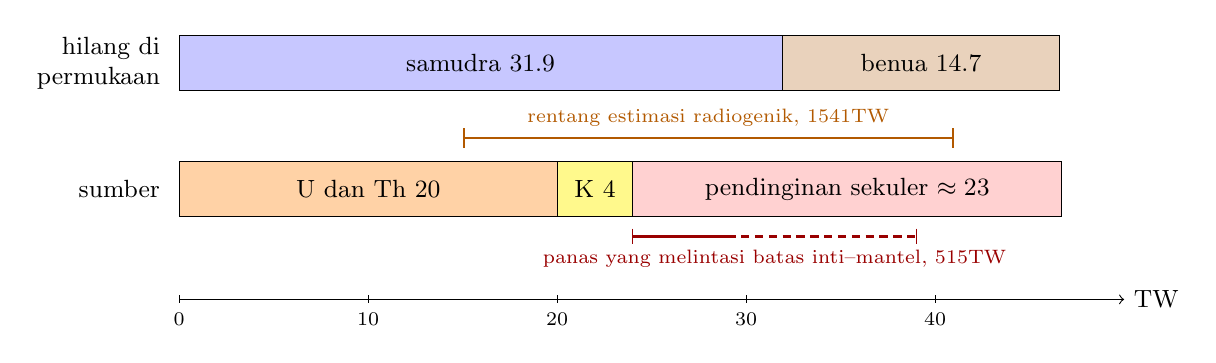
\begin{tikzpicture}[x=0.24cm, y=1cm, font=\small]
% ledger: dd10:split, kamland:2011, dye:radiogenic
% losses
\fill[blue!22] (0,1.6) rectangle (31.9,2.3);
\fill[brown!35] (31.9,1.6) rectangle (46.6,2.3);
\draw (0,1.6) rectangle (46.6,2.3);
\draw (31.9,1.6) -- (31.9,2.3);
\node at (15.95,1.95) {samudra 31.9};
\node at (39.25,1.95) {benua 14.7};
\node[anchor=east, align=right, font=\small] at (-0.5,1.95) {hilang di\\permukaan};
% sources
\fill[orange!35] (0,0) rectangle (20,0.7);
\fill[yellow!45] (20,0) rectangle (24,0.7);
\fill[red!18] (24,0) rectangle (46.7,0.7);
\draw (0,0) rectangle (46.7,0.7);
\draw (20,0) -- (20,0.7) (24,0) -- (24,0.7);
\node at (10,0.35) {U dan Th 20};
\node at (22,0.35) {K 4};
\node at (35.35,0.35) {pendinginan sekuler $\approx 23$};
\node[anchor=east, align=right] at (-0.5,0.35) {sumber};
% core part of secular cooling (range)
\draw[red!60!black, very thick] (24,-0.25) -- (29,-0.25);
\draw[red!60!black, thick, densely dashed] (29,-0.25) -- (39,-0.25);
\draw[red!60!black] (24,-0.15) -- (24,-0.35) (39,-0.15) -- (39,-0.35);
\node[anchor=north, font=\scriptsize, red!60!black] at (31.5,-0.3) {panas yang melintasi batas inti--mantel, \qtyrange{5}{15}{TW}};
% radiogenic range
\draw[|-|, orange!70!black, thick] (15,1.0) -- (41,1.0);
\node[anchor=south, font=\scriptsize, orange!70!black] at (28,1.02) {rentang estimasi radiogenik, \qtyrange{15}{41}{TW}};
% axis
\draw[->] (0,-1.05) -- (50,-1.05) node[right] {TW};
\foreach \x in {0,10,20,30,40} {\draw (\x,-1.0) -- (\x,-1.1) node[below, font=\scriptsize] {\x};}
\end{tikzpicture}

\par\smallskip{\small Anggaran panas Bumi. Atas: panas yang hilang melalui dasar samudra dan benua, \qty[uncertainty-mode=separate]{47 \pm 2}{TW} seluruhnya. Bawah: sumbernya, dengan bagian radiogenik uranium dan torium yang diukur oleh geoneutrino dan bagian kalium yang diperkirakan; sisanya, dengan selisih, adalah \omterm{def:b1:heat-budget:secular-cooling}{pendinginan sekuler}, yang sebagian kecil tidak diketahui disumbang oleh inti. Pita oranye menunjukkan rentang bagian radiogenik yang diizinkan oleh pengukuran geoneutrino.}
\label{fig:b1:heat-budget:budget}
\end{omfigure}

Panas radiogenik dahulu lebih besar, karena isotopnya lebih melimpah: \ce{^{235}U} dan \ce{^{40}K}, yang berumur pendek, ketika itu menyumbang jauh lebih banyak (Buku 2, kelas 12). Mesin panas Bumi perlahan kehabisan tenaga, pada kedua hitungan itu.

\section{Mengukur aliran panas}

\omterm{def:b1:heat-budget:heat-flow}{Aliran panas} tidak diukur secara langsung: ia dihitung dari gradien suhu dan konduktivitas.

\begin{proposition}[Hukum Fourier]\label{prop:b1:heat-budget:fourier}
Dalam medium dengan konduktivitas termal $k$, panas dikonduksikan menurun sepanjang gradien suhu dengan laju per satuan luas yang sebanding dengannya. Dengan $z$ kedalaman, dihitung positif ke bawah, dan $q$ dihitung positif ke atas,
\[
  q = k\,\frac{\mathrm dT}{\mathrm dz} .
\]
\end{proposition}
\admitted

Hukum ini ditetapkan dalam volume Sarjana Tahun ke-2 buku-buku fisika. Sebagian besar batuan menghantarkan panas pada \qtyrange{1.5}{3}{W.m^{-1}.K^{-1}} di bawah \qty{200}{\celsius}, lebih kecil ketika panas; model \omterm{def:b1:heat-budget:heat-flow}{aliran panas} benua memberikan \omterm{def:b1:layered-earth:layers}{kerak} atas granitik sekitar \qty{2.7}{W.m^{-1}.K^{-1}};
% ledger: delaney:conductivity, roy:granitic-k
gradien \qty{25}{K.km^{-1}} di dalamnya berarti \omterm{def:b1:heat-budget:heat-flow}{aliran panas} sekitar \qty{70}{mW.m^{-2}}.

Ketika batuan yang dilintasi sebuah lubang bor memiliki konduktivitas yang berbeda, gradiennya berubah dari satu batuan ke batuan berikutnya, tetapi \omterm{def:b1:heat-budget:heat-flow}{aliran panasnya} tidak, selama tidak ada panas yang dihasilkan atau tersimpan di antaranya. Proposisi berikut mengubah itu menjadi uji.

\begin{proposition}[Plot Bullard]\label{prop:b1:heat-budget:bullard}
Misalkan $R(z) = \int_0^z \mathrm d\zeta/k(\zeta)$ resistansi termal, per satuan luas, dari batuan antara permukaan dan kedalaman $z$, dalam \unit{m^2.K.W^{-1}}. Jika \omterm{def:b1:heat-budget:heat-flow}{aliran panas} $q$ sama di setiap kedalaman sebuah lubang bor, suhu merupakan fungsi linear dari resistansi termal: $T(z) = T_0 + q\,R(z)$.
\end{proposition}

\begin{proof}
Menurut hukum Fourier, $\mathrm dT/\mathrm dz = q/k(z)$. Mengintegralkan dari $0$ hingga
$z$ dengan $q$ konstan, $T(z) - T_0 = q\int_0^z \mathrm d\zeta/k(\zeta) = q\,R(z)$.
\end{proof}

\begin{method}[Aliran panas dari sebuah lubang bor]\label{met:b1:heat-budget:borehole}
\begin{enumerate}
  \item Catat suhu di sepanjang lubang bor jauh setelah pengeboran, ketika gangguan dari fluida pengebor sudah hilang, dan abaikan puluhan meter terdangkal, yang mengikuti musim.
  \item Ukur konduktivitas sampel inti dari setiap batuan yang dilintasi, di laboratorium, dan hitung resistansi termal $R(z)$ pada setiap kedalaman yang dicatat.
  \item Plot $T$ terhadap $R$: gradien garis lurus itu adalah \omterm{def:b1:heat-budget:heat-flow}{aliran panasnya}. Lengkungan menyingkapkan air yang mengalir melalui batuan, perubahan suhu permukaan di masa lalu, atau kesalahan pada suatu konduktivitas.
  \item Koreksi, bila perlu, untuk relief, yang membengkokkan isoterm di bawah bukit dan lembah, dan untuk pemanasan lambat sejak glasiasi terakhir, yang masih mengganggu kilometer teratas kira-kira.
\end{enumerate}
\end{method}

Di laut, lubang bor tidak diperlukan. Suhu di dasar samudra dalam sangat stabil, sehingga beberapa meter sedimen lunak sudah membawa gradien keseimbangan. Sebuah tombak baja yang membawa deretan sensor suhu dijatuhkan dari kapal dan ditancapkan ke dalam sedimen oleh beban berat (gambar di bawah); sensor-sensor itu merekam gradien, dan denyut panas yang dikirim sepanjang tombak memberikan konduktivitas sedimen di tempat.
Dasar samudra punya satu jebakan. Di \omterm{def:b1:layered-earth:layers}{kerak} muda, air laut bersirkulasi melalui basal yang retak dan membawa sebagian besar panas pergi melalui adveksi, sehingga \omterm{def:b1:heat-budget:heat-flow}{aliran panas} konduktif yang terukur jauh lebih kecil daripada kehilangan sebenarnya. Kehilangan melalui dasar samudra termuda karena itu dihitung dari model pendinginan pada \cref{sec:b1:heat-budget:boundary-layer}, dikalibrasi pada \omterm{def:b1:layered-earth:layers}{kerak} tua tempat sirkulasi telah berhenti: bagian yang dihitung ini, \qty{23.1}{TW}, 
kira-kira separuh dari total global. % ledger: dd10:young-ocean

\begin{omfigure}
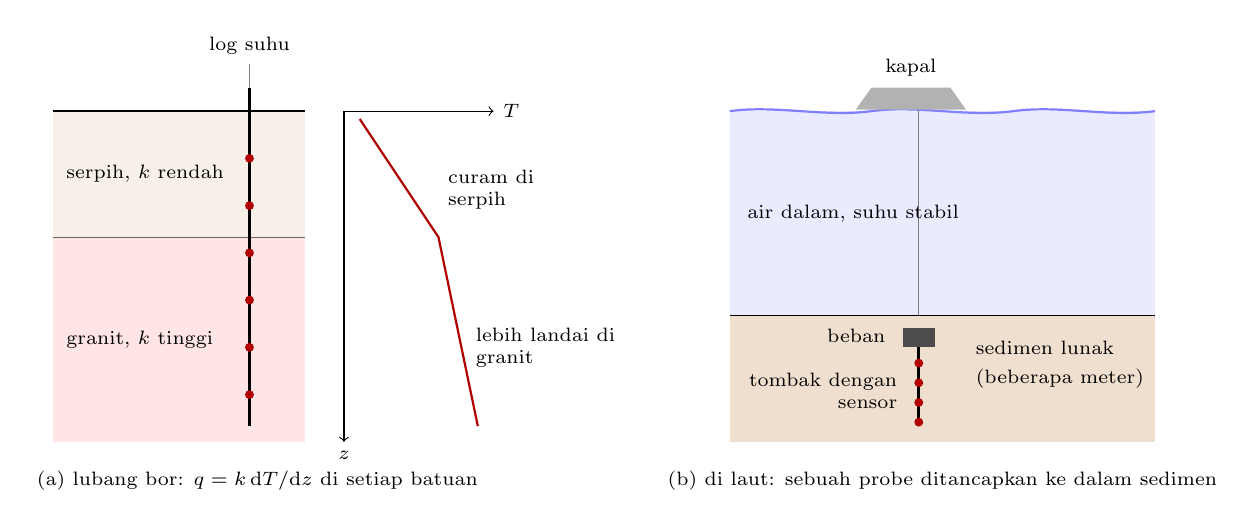
\begin{tikzpicture}[font=\scriptsize, x=1cm, y=1cm]
% --- left: borehole on land ---
\fill[brown!12] (0,0) rectangle (3.2,-1.6);
\fill[red!10] (0,-1.6) rectangle (3.2,-4.2);
\draw[thick] (0,0) -- (3.2,0);
\node[anchor=west] at (0.05,-0.8) {serpih, $k$ rendah};
\node[anchor=west] at (0.05,-2.9) {granit, $k$ tinggi};
\draw[black!60] (0,-1.6) -- (3.2,-1.6);
\draw[very thick] (2.5,0.3) -- (2.5,-4.0);
\draw[gray] (2.5,0.6) -- (2.5,0.3);
\foreach \y in {-0.6,-1.2,-1.8,-2.4,-3.0,-3.6} {\fill[red!70!black] (2.5,\y) circle (1.6pt);}
\node[anchor=south] at (2.5,0.6) {log suhu};
% inset T(z)
\draw[->] (3.7,0) -- (5.6,0) node[right] {$T$};
\draw[->] (3.7,0) -- (3.7,-4.2) node[below] {$z$};
\draw[thick, red!70!black] (3.9,-0.1) -- (4.9,-1.6) -- (5.4,-4.0);
\node[anchor=west, align=left] at (4.9,-1.0) {curam di\\serpih};
\node[anchor=west, align=left] at (5.25,-3.0) {lebih landai di\\granit};
\node[anchor=north] at (2.6,-4.45) {(a) lubang bor: $q = k\,\mathrm dT/\mathrm dz$ di setiap batuan};
% --- right: probe at sea ---
\begin{scope}[xshift=8.6cm]
\fill[blue!8] (0,0) rectangle (5.4,-2.6);
\draw[blue!50, thick] (0,0) .. controls (0.6,0.08) and (1.2,-0.08) .. (1.8,0)
  .. controls (2.4,0.08) and (3.0,-0.08) .. (3.6,0) .. controls (4.2,0.08) and (4.8,-0.08) .. (5.4,0);
\fill[gray!60] (1.6,0.02) -- (3.0,0.02) -- (2.8,0.3) -- (1.8,0.3) -- cycle;
\node[anchor=south] at (2.3,0.32) {kapal};
\draw[gray] (2.4,0.02) -- (2.4,-2.75);
\fill[brown!25] (0,-2.6) rectangle (5.4,-4.2);
\draw (0,-2.6) -- (5.4,-2.6);
\node[anchor=west] at (3.0,-3.0) {sedimen lunak};
\node[anchor=west] at (3.0,-3.4) {(beberapa meter)};
\fill[black!70] (2.2,-2.75) rectangle (2.6,-3.0);
\draw[very thick] (2.4,-3.0) -- (2.4,-4.0);
\foreach \y in {-3.2,-3.45,-3.7,-3.95} {\fill[red!70!black] (2.4,\y) circle (1.6pt);}
\node[anchor=east, align=right] at (2.1,-2.85) {beban};
\node[anchor=east, align=right] at (2.25,-3.55) {tombak dengan\\sensor};
\node[anchor=west] at (0.1,-1.3) {air dalam, suhu stabil};
\node[anchor=north] at (2.7,-4.45) {(b) di laut: sebuah probe ditancapkan ke dalam sedimen};
\end{scope}
\end{tikzpicture}

\par\smallskip{\small Mengukur \omterm{def:b1:heat-budget:heat-flow}{aliran panas} (skematis, tidak sesuai skala). (a) Di darat, suhu dicatat di sepanjang lubang bor setelah kembali ke keseimbangan, dan konduktivitas tiap batuan diukur pada inti: gradiennya lebih curam di tempat konduktivitasnya lebih rendah, dan \omterm{def:b1:heat-budget:heat-flow}{aliran panas}, hasil kali keduanya, sama. (b) Di laut, sebuah tombak dengan sensor ditancapkan beberapa meter ke dalam sedimen dasar samudra.}
\label{fig:b1:heat-budget:measure}
\end{omfigure}

\begin{inthefield}[Aliran panas di laut]
\begin{minipage}[t]{0.55\linewidth}\vspace{0pt}
Di kapal riset, probe \omterm{def:b1:heat-budget:heat-flow}{aliran panas} adalah tombak berat yang digantung dari derek buritan. Ia diturunkan dengan kabel kapal hingga tepat di atas dasar laut, lalu dilepas: beban itu menancapkannya ke dalam sedimen, dan kru menunggu di dek sementara sensor menyesuaikan diri dengan suhu lumpur, lalu menariknya keluar dan pindah ke stasiun berikutnya yang tidak jauh. Sederet stasiun semacam itu melintasi sisi punggungan memberikan penurunan \omterm{def:b1:heat-budget:heat-flow}{aliran panas} terhadap umur dasar samudra, dan sebaran antara stasiun-stasiun yang bertetangga menunjukkan di mana air mengalir melalui \omterm{def:b1:layered-earth:layers}{kerak} di bawahnya.
\end{minipage}\hfill
\begin{minipage}[t]{0.42\linewidth}\vspace{0pt}
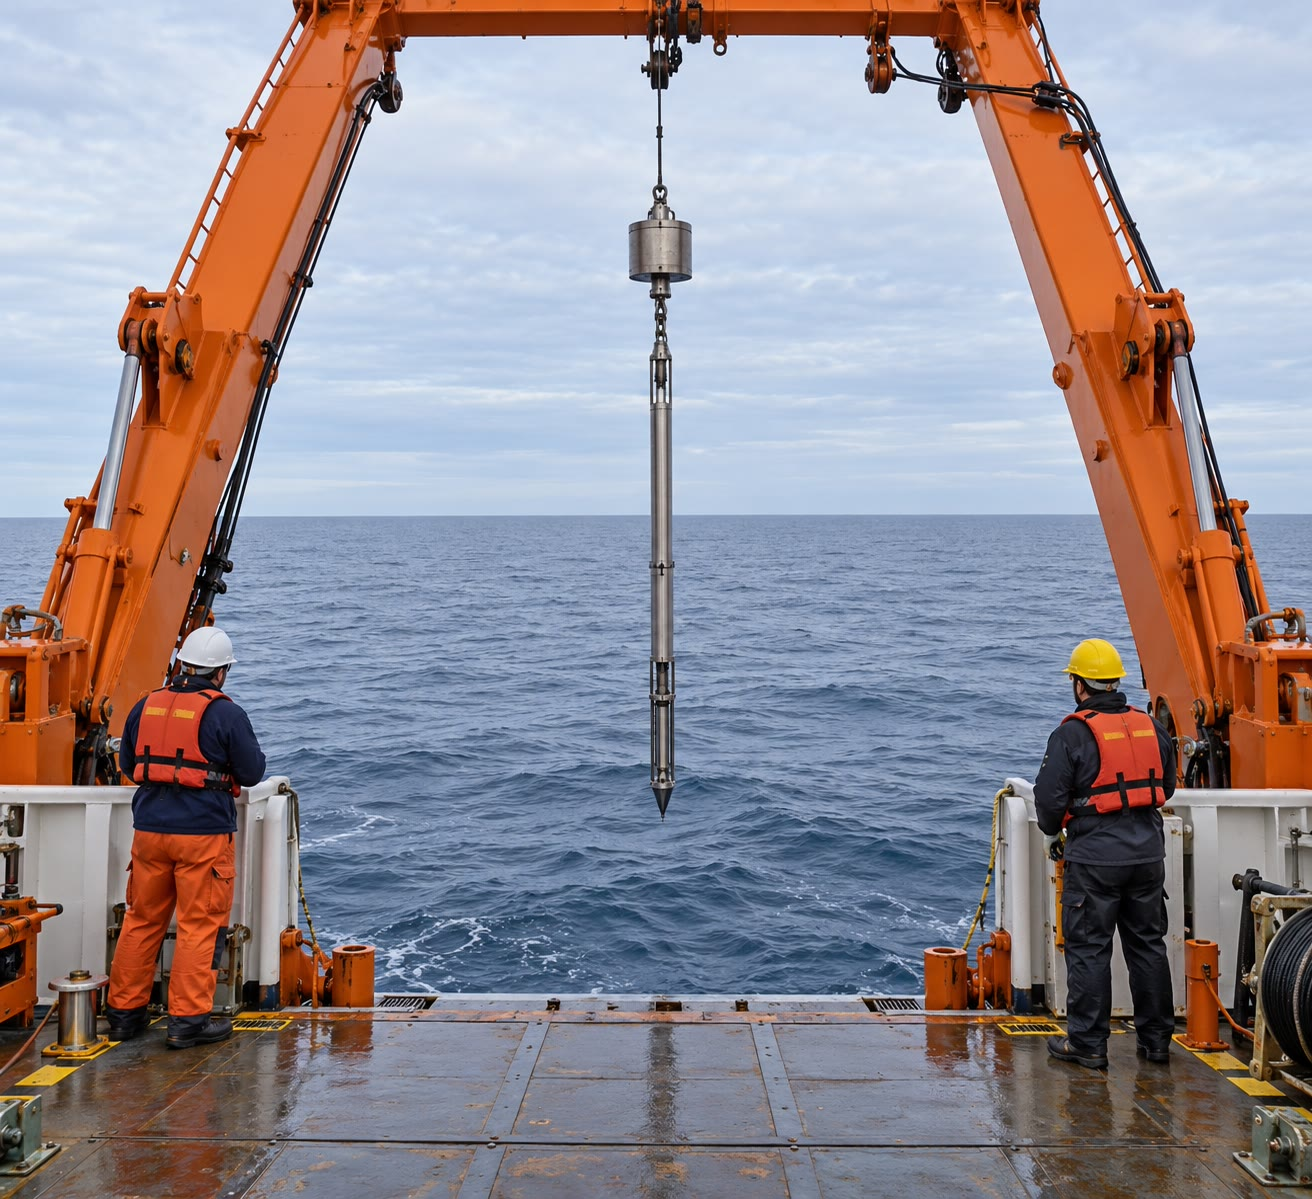
\includegraphics[width=\linewidth]{images/book3/ai/b1-heatflow-probe.jpg}

{\scriptsize Probe \omterm{def:b1:heat-budget:heat-flow}{aliran panas} yang tergantung dari derek buritan sebuah kapal riset (ilustrasi buatan AI).}
\end{minipage}
\end{inthefield}

\section{Geoterm mantap secara konduktif}

\begin{definition}[Geoterm]\label{def:b1:heat-budget:geotherm}
\emph{Geoterm}\index{geoterm} di bawah suatu titik permukaan adalah suhu sebagai fungsi kedalaman di sana, $T(z)$. Ia adalah geoterm konduktif yang mantap ketika tidak berubah terhadap waktu dan panas dibawa sepanjang itu oleh konduksi saja.
\end{definition}

Di dalam \omterm{def:b1:layered-earth:lithosphere}{litosfer}, jauh dari gunung api aktif dan dari sirkulasi air, panas dibawa oleh konduksi, dan dalam skala jutaan tahun \omterm{def:b1:heat-budget:geotherm}{geoterm} itu mantap. Bentuknya kemudian mengikuti dari keseimbangan energi.

\begin{theorem}[Konduksi mantap dengan produksi panas]\label{thm:b1:heat-budget:balance}
Sepanjang \omterm{def:b1:heat-budget:geotherm}{geoterm} konduktif yang mantap, dalam medium dengan konduktivitas seragam $k$, dengan produksi panas $A(z)$ dan tanpa \omterm{def:b1:heat-budget:heat-flow}{aliran panas} horizontal,
\[
  \frac{\mathrm dq}{\mathrm dz} = -A(z), \qquad\text{yaitu}\qquad
  k\,\frac{\mathrm d^2T}{\mathrm dz^2} = -A(z).
\]
\end{theorem}

\begin{proof}
Pertimbangkan lempeng horizontal dengan luas $S$ di antara kedalaman $z$ dan $z +
\mathrm dz$. Panas masuk melalui dasarnya dengan laju $q(z + \mathrm dz)\,S$,
keluar melalui puncaknya dengan laju $q(z)\,S$, dan dihasilkan di dalamnya dengan
laju $A(z)\,S\,\mathrm dz$. Dalam keadaan mantap tidak ada panas yang tersimpan, sehingga
$q(z)\,S = q(z + \mathrm dz)\,S + A(z)\,S\,\mathrm dz$, yang memberikan
$\mathrm dq/\mathrm dz = -A$. Menurut hukum Fourier $q = k\,\mathrm dT/\mathrm dz$,
dan dengan $k$ seragam, $k\,T'' = -A$.
\end{proof}

Dibaca dari permukaan ke bawah, \omterm{def:b1:heat-budget:heat-flow}{aliran panas} berkurang terhadap kedalaman sebesar panas yang dihasilkan di atas setiap level: apa yang melintasi permukaan adalah panas yang datang dari bawah ditambah semua panas yang dihasilkan sepanjang jalan. Dua distribusi $A$ memberikan bentuk tertutup.

\begin{proposition}[Lapisan radiogenik seragam]\label{prop:b1:heat-budget:uniform}
Misalkan produksi panas adalah $A$ dari permukaan hingga kedalaman $h$ dan nol di bawahnya, permukaan berada pada suhu $T_0$, dan \omterm{def:b1:heat-budget:heat-flow}{aliran panas} permukaan adalah $q_0$.
Maka untuk $0 \le z \le h$
\[
  q(z) = q_0 - A z, \qquad T(z) = T_0 + \frac{q_0 z}{k} - \frac{A z^2}{2k},
\]
dan di bawah $h$ \omterm{def:b1:heat-budget:heat-flow}{aliran panas} seragam, $q_m = q_0 - A h$, dan \omterm{def:b1:heat-budget:geotherm}{geoterm} berupa garis lurus dengan gradien $q_m/k$.
\end{proposition}

\begin{proof}
Integrasikan $\mathrm dq/\mathrm dz = -A$ dari $0$ dengan $q(0) = q_0$: $q = q_0 -
Az$. Maka $\mathrm dT/\mathrm dz = (q_0 - Az)/k$; mengintegralkan dengan $T(0) = T_0$
memberikan parabola. Di bawah $h$, $\mathrm dq/\mathrm dz = 0$ dan $q$ mempertahankan nilainya pada $h$.
\end{proof}

\begin{theorem}[Produksi panas eksponensial dan hubungan aliran panas linear]
\label{thm:b1:heat-budget:exponential}
Misalkan produksi panas berkurang terhadap kedalaman sebagai $A(z) = A_0 e^{-z/D}$, \omterm{def:b1:heat-budget:heat-flow}{aliran panas} mendekati $q_m$ pada kedalaman besar, dan permukaan berada pada $T_0$. Maka
\[
  q(z) = q_m + A_0 D\,e^{-z/D}, \qquad
  T(z) = T_0 + \frac{q_m z}{k} + \frac{A_0 D^2}{k}\bigl(1 - e^{-z/D}\bigr),
\]
dan \omterm{def:b1:heat-budget:heat-flow}{aliran panas} permukaan adalah
\[
  q_0 = q_m + A_0 D .
\]
\end{theorem}

\begin{proof}
Dari \cref{thm:b1:heat-budget:balance}, $\mathrm dq/\mathrm dz =
-A_0e^{-z/D}$, sehingga $q(z) = A_0 D e^{-z/D} + C$; ketika $z \to \infty$, $q \to C$,
maka $C = q_m$. Pada $z = 0$, $q_0 = q_m + A_0 D$. Lalu $\mathrm dT/\mathrm dz =
q/k = q_m/k + (A_0D/k)\,e^{-z/D}$, dan mengintegralkan dari $0$ dengan $T(0) = T_0$,
$T = T_0 + q_m z/k + (A_0 D^2/k)(1 - e^{-z/D})$.
\end{proof}

Baris terakhir adalah prediksi yang dapat diuji di permukaan. Pluton granit di satu wilayah memiliki \omterm{def:b1:heat-budget:heat-flow}{aliran panas} dalam $q_m$ yang sama dan, jika mereka berbeda hanya dalam seberapa kaya mereka akan uranium, torium dan kalium, skala yang sama $D$; maka \omterm{def:b1:heat-budget:heat-flow}{aliran panas} yang diukur di atas setiap pluton seharusnya merupakan fungsi linear dari produksi panas yang diukur pada batuannya, dengan gradien $D$, suatu panjang, dan intersep $q_m$, \omterm{def:b1:heat-budget:heat-flow}{aliran panas} tereduksi, yang berasal dari bawah lapisan radiogenik. Francis Birch pertama kali mengamati garis semacam itu, yang dilaporkan pada 1968, dan pada tahun yang sama tiga provinsi didefinisikan menurut garisnya:
\begin{center}
\small
% ledger: roy:provinces, roy:linear-relation
\begin{tabular}{lcc}
\hline
provinsi & intersep $q_m$ (\unit{mW.m^{-2}}) & gradien $D$ (\unit{km}) \\
\hline
Amerika Serikat timur & 33 & 7.5 \\
Provinsi Basin and Range & 59 & 9.4 \\
Sierra Nevada & 17 & 10 \\
\hline
\end{tabular}
\end{center}
Intersep-intersep, yang diterbitkan sebagai 0.8, 1.4 dan $0.4\times\qty{e-6}{cal.cm^{-2}.s^{-1}}$, dikonversi dengan $\qty{1}{\micro cal.cm^{-2}.s^{-1}} = \qty{41.84}{mW.m^{-2}}$ (\cref{exo:b1:heat-budget:4}). Gradien hanya sedikit bervariasi, dari 7 hingga \qty{10}{km}; \omterm{def:b1:heat-budget:heat-flow}{aliran panas} tereduksi bervariasi banyak, dan peta-petanya menunjukkan di mana \omterm{def:b1:layered-earth:layers}{mantel} di bawahnya panas, seperti di bawah \omterm{def:b1:layered-earth:layers}{kerak} yang meregang di Basin and Range. Lapisan seragam dari \cref{prop:b1:heat-budget:uniform} juga memberikan garis lurus, dengan gradien $h$: kedua model cocok dengan data, tetapi hanya model eksponensial yang tetap berupa garis lurus dengan gradien yang sama ketika pluton tererosi pada kedalaman yang berbeda (\cref{exo:b1:heat-budget:10}), itulah sebabnya ia lebih disukai.

\begin{omfigure}
\begin{tikzpicture}
\begin{axis}[omdepth, width=0.82\linewidth, height=8.6cm, xmin=0, xmax=1800, ymin=0, ymax=250, axis x line=top, axis y line=left, axis line style={-}, clip=true,
  xlabel={suhu (\unit{\degreeCelsius})}, ylabel={kedalaman (km)},
  tick label style={font=\scriptsize}, label style={font=\small},
  legend style={font=\scriptsize, at={(0.02,0.02)}, anchor=south west, draw=none, fill=white, fill opacity=0.85, text opacity=1},
  legend cell align=left]
\addplot[very thick, black!45] table[x=T, y=depth] {figdata/out/bachelor-1-geotherms-adiabat.dat};
\addlegendentry{adiabat mantel}
\addplot[very thick, red!75!black] table[x=T45, y=depth] {figdata/out/bachelor-1-geotherms-continental.dat};
\addlegendentry{$q_0 = \qty{70}{mW.m^{-2}}$}
\addplot[very thick, orange!80!black] table[x=T30, y=depth] {figdata/out/bachelor-1-geotherms-continental.dat};
\addlegendentry{$q_0 = \qty{55}{mW.m^{-2}}$}
\addplot[very thick, green!45!black] table[x=T15, y=depth] {figdata/out/bachelor-1-geotherms-continental.dat};
\addlegendentry{$q_0 = \qty{40}{mW.m^{-2}}$}
\addplot[thick, blue!70!black, densely dashdotted] table[x=T, y=depth] {figdata/out/bachelor-1-geotherms-oceanic.dat};
\addlegendentry{dasar samudra berumur \qty{60}{Ma}}
\addplot[thin, dashed, red!75!black, forget plot] table[x=Tc45, y=depth] {figdata/out/bachelor-1-geotherms-continental.dat};
\addplot[thin, dashed, orange!80!black, forget plot] table[x=Tc30, y=depth] {figdata/out/bachelor-1-geotherms-continental.dat};
\addplot[thin, dashed, green!45!black, forget plot] table[x=Tc15, y=depth] {figdata/out/bachelor-1-geotherms-continental.dat};
\draw[densely dotted, black!60] (axis cs:0,35) -- (axis cs:1800,35);
\node[font=\scriptsize, anchor=south east] at (axis cs:1790,35) {Moho, \qty{35}{km}};
\fill (axis cs:1384.0,70.8) circle (1.6pt);
\fill (axis cs:1403.2,107.8) circle (1.6pt);
\fill (axis cs:1459.7,224.9) circle (1.6pt);
\node[font=\scriptsize, anchor=west] at (axis cs:1420,66) {\qty{71}{km}};
\node[font=\scriptsize, anchor=west] at (axis cs:1440,104) {\qty{108}{km}};
\node[font=\scriptsize, anchor=west] at (axis cs:1495,222) {\qty{225}{km}};
\end{axis}
\end{tikzpicture}

\par\smallskip{\small \omterm{def:b1:heat-budget:geotherm}{Geoterm} konduktif mantap benua dengan produksi panas $A_0 = \qty{2.5}{\micro W.m^{-3}}$ yang berkurang sepanjang $D = \qty{10}{km}$, $k = \qty{2.5}{W.m^{-1}.K^{-1}}$, untuk tiga \omterm{def:b1:heat-budget:heat-flow}{aliran panas} permukaan (\omterm{def:b1:heat-budget:heat-flow}{aliran panas} tereduksi 15, 30 dan \qty{45}{mW.m^{-2}}). Setiap \omterm{def:b1:heat-budget:geotherm}{geoterm} mengikuti kurva konduktifnya (putus-putus di luar) hingga \omterm{def:b1:heat-budget:adiabat}{adiabat mantel}, yang ditemuinya pada titik: dasar \omterm{def:b1:heat-budget:boundary-layer}{litosfer termal}. \omterm{def:b1:heat-budget:geotherm}{Geoterm} dasar samudra adalah \omterm{def:b1:heat-budget:geotherm}{geoterm} setengah-ruang yang didinginkan selama \qty{60}{Ma}. Konduktivitas seragam adalah penyederhanaan.}
\label{fig:b1:heat-budget:geotherms}
\end{omfigure}

\begin{method}[Suhu pada kedalaman di bawah pluton]\label{met:b1:heat-budget:moho}
\begin{enumerate}
  \item Ukur \omterm{def:b1:heat-budget:heat-flow}{aliran panas} permukaan $q_0$ di atas pluton (metode lubang bor) dan produksi panasnya $A_0$ dari kandungan U, Th dan K-nya.
  \item Dari garis provinsi, atau dengan nilai $D$ sekitar \qty{10}{km}, hitung $q_m = q_0 - A_0 D$.
  \item Terapkan \cref{thm:b1:heat-budget:exponential}. Di bawah beberapa kali $D$, $e^{-z/D}$ dapat diabaikan dan \omterm{def:b1:heat-budget:geotherm}{geoterm} berupa garis lurus $T_0 + A_0D^2/k + q_m z/k$: lapisan radiogenik telah menaikkan setiap suhu dalam sebesar $A_0D^2/k$.
\end{enumerate}
\end{method}

Pada gambar, suhu di \omterm{def:b1:layered-earth:discontinuity}{Moho} berkisar dari sekitar \qty{320}{\degreeCelsius} untuk \omterm{def:b1:heat-budget:heat-flow}{aliran panas} terendah hingga lebih dari \qty{700}{\degreeCelsius} untuk yang tertinggi: \omterm{def:b1:heat-budget:heat-flow}{aliran panas} di permukaan memuat pembacaan langsung suhu \omterm{def:b1:layered-earth:layers}{kerak} dalam, yang mengatur kekuatannya (\cref{ch:b1:stress-strain-rheology}).

\section{Konduksi melawan konveksi}

Konduksi lambat. Seberapa lambat itu mengikuti dari persamaan panas, yang diturunkan buku-buku fisika dari hukum Fourier dan keseimbangan \cref{thm:b1:heat-budget:balance} dengan penyimpanan ditambahkan: dalam satu dimensi, tanpa produksi panas,
$\partial T/\partial t = \kappa\,\partial^2 T/\partial z^2$.

\begin{proposition}[Skala waktu konduktif]\label{prop:b1:heat-budget:timescale}
Perubahan suhu yang dikenakan pada batas suatu benda konduktif menyebar sepanjang jarak $L$ dalam waktu berorde
\[
  \tau = \frac{L^2}{\kappa} .
\]
\end{proposition}

\begin{proof}
Tulis $z = L z^*$, $t = \tau t^*$, dengan $z^*$ dan $t^*$ tak berdimensi. Persamaan panas menjadi $\partial T/\partial t^* = (\kappa\tau/L^2)\,\partial^2
T/\partial z^{*2}$. Solusinya bervariasi pada skala $z^* \sim 1$ ketika $t^* \sim 1$ hanya jika koefisiennya berorde satu, yaitu jika $\tau \sim L^2/\kappa$.
\end{proof}

Batuan memiliki $\kappa \approx \qty{e-6}{m^2.s^{-1}}$. Siklus suhu harian mencapai beberapa puluh sentimeter ke dalam tanah, yang tahunan beberapa meter, dan pemanasan sejak glasiasi terakhir sekitar satu kilometer. Melintasi \omterm{def:b1:layered-earth:lithosphere}{litosfer} setebal \qty{100}{km}, $\tau = \qty{e16}{s}$, sekitar \qty{300}{Ma}. Melintasi \omterm{def:b1:layered-earth:layers}{mantel} setebal \qty{2900}{km}, $\tau = \qty{8.4e18}{s}$, atau \qty{270}{Ga}: enam puluh kali umur Bumi, \qty{4.54}{Ga}. % ledger: england:kelvin, usgs:age-earth
Konduksi saja tidak mungkin membawa panas \omterm{def:b1:layered-earth:layers}{mantel} dalam ke dekat permukaan. \omterm{def:b1:layered-earth:layers}{Mantel} berkonveksi, dan di bagian dalamnya panas dibawa oleh gerakan batuan itu sendiri, dengan kecepatan lempeng, sentimeter per tahun. % ledger: usgs:san-andreas

\begin{definition}[Adiabat mantel]\label{def:b1:heat-budget:adiabat}
\emph{Adiabat mantel}\index{adiabat mantel} adalah \omterm{def:b1:heat-budget:geotherm}{geoterm} dari bagian dalam yang tercampur baik dari \omterm{def:b1:layered-earth:layers}{mantel} yang berkonveksi: suhu yang diambil batuan \omterm{def:b1:layered-earth:layers}{mantel} ketika ia naik atau turun cukup cepat untuk tidak bertukar panas dengan sekelilingnya, mendingin karena ekspansi ketika ia naik dan menghangat karena kompresi ketika ia turun.
\end{definition}

Termodinamika memberikan gradiennya, $\mathrm dT/\mathrm dz = \alpha g T/c_p$, dengan $\alpha$ ekspansivitas termal dan $c_p$ kalor jenis (fisika, diterima di sini). Gradien itu kecil. Evaluasi terkini dari fisika \omterm{def:b1:rock-forming-minerals:mineral}{mineral} memberikan \qty{0.54}{K.km^{-1}} pada kedalaman \qty{50}{km}, menurun menjadi \qty{0.36}{K.km^{-1}} pada \qty{410}{km}, lalu 0.41 hingga \qty{0.23}{K.km^{-1}} melalui \omterm{def:b1:layered-earth:layers}{mantel} bawah, dengan \qty{1646}{K} pada \qty{50}{km} dan \qty{2587}{K} pada \qty{2800}{km}.
% ledger: katsura:adiabat
Diekstrapolasi ke permukaan, adiabat memberikan suhu potensial \omterm{def:b1:layered-earth:layers}{mantel}, \qty{1619}{K} atau sekitar \qty{1350}{\degreeCelsius}: suhu yang akan dimiliki \omterm{def:b1:layered-earth:layers}{mantel} jika dibawa naik ke permukaan tanpa bertukar panas. Konsep suhu potensial didefinisikan, untuk atmosfer dan samudra, dalam \cref{ch:b1:fluid-envelopes-structure}. Suhu yang naik hanya \qty{0.5}{K} per kilometer sementara \omterm{def:b1:heat-budget:geotherm}{geoterm} konduktif dekat permukaan naik sebesar \qty{25}{K} adalah tanda konveksi.

\begin{history}[John Perry dan Bumi yang mendingin]
Pada 1862--1863 William Thomson, kemudian Lord Kelvin, menghitung umur Bumi dari pendinginannya. Ia memperlakukannya sebagai padatan yang mendingin secara konduktif dari suhu seragam sekitar \qty{3900}{\degreeCelsius}; dengan gradien rata-rata masa itu yang ia pilih dari pengukuran zamannya, sekitar \qty{36}{K.km^{-1}}, dan difusivitas \qty{1.2e-6}{m^2.s^{-1}}, waktu yang diperlukan untuk mencapai gradien hari ini sekitar \qty{96}{Ma}, di antara batas 24 dan \qty{400}{Ma} (\cref{exo:b1:heat-budget:9}). Para ahli geologi menemukan angka itu jauh terlalu pendek. Pada 1895, setahun sebelum radioaktivitas ditemukan, mantan asistennya John Perry menunjuk sebuah asumsi lain: jika bagian dalam sebagian cair dan berkonveksi, ia akan membawa panas seolah-olah memiliki konduktivitas yang sangat besar, dan seluruh bagian dalam, bukan cangkang luar yang tipis, akan memberi makan \omterm{def:b1:heat-budget:heat-flow}{aliran panas} permukaan. Argumennya diabaikan dan dilupakan; konveksi \omterm{def:b1:layered-earth:layers}{mantel}, yang ditetapkan jauh kemudian, membuktikan dirinya benar: \omterm{def:b1:layered-earth:layers}{mantel} dalam mendingin dengan konveksi, dan itulah \omterm{def:b1:heat-budget:secular-cooling}{pendinginan sekuler} dalam anggaran. % ledger: england:kelvin, england:perry
\end{history}

\begin{proposition}[Bumi teraduk baik menurut Perry]\label{prop:b1:heat-budget:perry}
Misalkan sebuah bola dengan jari-jari $R$ memiliki bagian dalam yang teraduk baik pada suhu seragam $T_i(t)$, dengan kapasitas panas $\rho c$ per satuan volume, di bawah tutup konduktif setebal $L \ll R$ dan konduktivitas $k$ yang permukaannya berada pada $\qty{0}{\degreeCelsius}$, dan misalkan tidak ada produksi panas. Maka
\[
  T_i(t) = T_i(0)\,e^{-t/\tau_P}, \qquad \tau_P = \frac{RL}{3\kappa},
\]
dan \omterm{def:b1:heat-budget:heat-flow}{aliran panas} permukaan $kT_i/L$ meluruh dengan konstanta waktu yang sama.
\end{proposition}

\begin{proof}
Karena tutupnya tipis, ia berada dalam keadaan mantap dan membawa \omterm{def:b1:heat-budget:heat-flow}{aliran panas}
$q = kT_i/L$. Bagian dalam kehilangan panasnya melalui luas $4\pi R^2$:
$\tfrac43\pi R^3\rho c\,\mathrm dT_i/\mathrm dt = -4\pi R^2 kT_i/L$, yaitu
$\mathrm dT_i/\mathrm dt = -3\kappa T_i/(RL)$ dengan $\kappa = k/(\rho c)$, yang solusinya adalah eksponensial dengan $\tau_P = RL/(3\kappa)$.
\end{proof}

Untuk $R = \qty{6400}{km}$, $L = \qty{100}{km}$ dan $\kappa =
\qty{e-6}{m^2.s^{-1}}$, $\tau_P = \qty{6.8}{Ga}$: Bumi yang berkonveksi mempertahankan \omterm{def:b1:heat-budget:heat-flow}{aliran panas} tinggi selama miliaran tahun, sedangkan Bumi konduktif Kelvin kehilangannya dalam puluhan juta tahun (\cref{exo:b1:heat-budget:11}).

\section{Litosfer sebagai lapisan batas termal}\label{sec:b1:heat-budget:boundary-layer}

\begin{definition}[Lapisan batas termal, litosfer termal]\label{def:b1:heat-budget:boundary-layer}
Dalam fluida yang berkonveksi, \emph{lapisan batas termal}\index{lapisan batas termal} adalah lapisan di sepanjang suatu batas tempat panas melintas secara konduktif dan suhunya berubah dari suhu batas ke suhu bagian dalam yang tercampur baik. \emph{Litosfer termal}\index{litosfer termal} adalah lapisan batas termal atas \omterm{def:b1:layered-earth:layers}{mantel}: cangkang luar Bumi dari permukaan ke bawah hingga kedalaman tempat \omterm{def:b1:heat-budget:geotherm}{geoterm} konduktif bertemu \omterm{def:b1:heat-budget:adiabat}{adiabat mantel}.
\end{definition}

Lempeng-lempeng adalah bagian atas dingin dari konveksi \omterm{def:b1:layered-earth:layers}{mantel}, lapisan batas atasnya. Dasarnya, tempat \omterm{def:b1:heat-budget:geotherm}{geoterm} konduktif yang curam membengkok menjadi adiabat yang landai, berada pada \qtyrange{70}{230}{km} dalam gambar \omterm{def:b1:heat-budget:geotherm}{geoterm} untuk \omterm{def:b1:heat-budget:heat-flow}{aliran panas} benua dari 70 hingga \qty{40}{mW.m^{-2}}, dalam rentang yang diukur seismologi (\cref{ch:b1:layered-earth}): \omterm{def:b1:layered-earth:lithosphere}{litosfer} yang didefinisikan oleh kekuatannya dan \omterm{def:b1:layered-earth:lithosphere}{litosfer} yang didefinisikan oleh suhunya kira-kira merupakan cangkang yang sama, karena kekuatan bergantung pada suhu. Di dasar \omterm{def:b1:layered-earth:layers}{mantel}, lapisan D$''$ adalah lapisan batas bawah, dipanaskan dari bawah oleh inti.

Di bawah samudra, lapisan batas lahir di punggungan, tempat \omterm{def:b1:layered-earth:layers}{mantel} panas naik ke permukaan, dan menebal ketika lempeng menjauh dan mendingin. Pendinginan setengah-ruang dari suhu seragam, yang diselesaikan oleh Fourier dan dipakai oleh Kelvin untuk seluruh Bumi, menggambarkannya dengan baik (\cref{ch:b1:rifts-ridges-margins} dan volume Sarjana Tahun ke-3 menurunkannya): isoterm menjadi lebih dalam sebanding dengan akar kuadrat umur dasar (gambar di bawah), dan \omterm{def:b1:heat-budget:heat-flow}{aliran panas} berkurang sebagai
\[
  q(t) = \frac{C}{\sqrt t}, \qquad C \approx \qty{490}{mW.m^{-2}.Ma^{1/2}},
\]
nilai yang dipakai dalam anggaran global. % ledger: dd10:young-ocean
Pada \qty{100}{Ma} setengah-ruang telah mendingin hingga sekitar \qty{130}{km} (\cref{exo:b1:heat-budget:12}). Lempeng yang sebenarnya berhenti menebal lebih cepat: gelombang seismik yang melintasi Pasifik paling baik dicocokkan oleh lempeng yang mendingin dan cenderung menuju ketebalan \qtyrange{85}{95}{km}, perataan dasar laut tua yang dijumpai lagi di \cref{ch:b1:rifts-ridges-margins}.
% ledger: fischer:lithosphere

Anggaran panas, \omterm{def:b1:heat-budget:heat-flow}{aliran panas} dan struktur termal lempeng bersatu dalam bab-bab berikutnya: lempeng yang mendingin tenggelam (\cref{ch:b1:rifts-ridges-margins}), dan \omterm{def:b1:layered-earth:lithosphere}{litosfer} dingin yang tenggelam di zona subduksi adalah bagian turun dari konveksi yang menjadi miliknya.

\begin{omfigure}
\begin{tikzpicture}
\begin{axis}[width=0.86\linewidth, height=5.6cm, xmin=0, xmax=100, ymin=0, ymax=170,
  y dir=reverse, axis x line=top, axis y line=left, axis line style={-}, clip=false,
  xlabel={umur dasar samudra (Ma), bertambah dengan jarak dari punggungan},
  ylabel={kedalaman (km)}, tick label style={font=\scriptsize}, label style={font=\small}]
\addplot[fill=blue!12, draw=none] table[x=age, y=z1200] {figdata/out/bachelor-1-geotherms-isotherms.dat} \closedcycle;
\addplot[thick, blue!30!black] table[x=age, y=z400] {figdata/out/bachelor-1-geotherms-isotherms.dat};
\addplot[thick, blue!50!red] table[x=age, y=z800] {figdata/out/bachelor-1-geotherms-isotherms.dat};
\addplot[very thick, red!75!black] table[x=age, y=z1200] {figdata/out/bachelor-1-geotherms-isotherms.dat};
\node[font=\scriptsize, anchor=south, fill=blue!12, inner sep=1pt] at (axis cs:80,24) {\qty{400}{\degreeCelsius}};
\node[font=\scriptsize, anchor=south, fill=blue!12, inner sep=1pt] at (axis cs:80,55) {\qty{800}{\degreeCelsius}};
\node[font=\scriptsize, anchor=south, fill=blue!12, inner sep=1pt] at (axis cs:80,108) {\qty{1200}{\degreeCelsius}};
\node[font=\small] at (axis cs:60,72) {litosfer termal};
\node[font=\small] at (axis cs:55,150) {mantel berkonveksi, sekitar \qty{1350}{\degreeCelsius}};
\draw[->, thick, red!60!black] (axis cs:3,165) -- (axis cs:3,125);
\node[font=\scriptsize, anchor=west, red!60!black] at (axis cs:4,140) {naik di bawah punggungan};
\draw[->, thick, black!60] (axis cs:30,5) -- (axis cs:70,5);
\node[font=\scriptsize, anchor=west] at (axis cs:70,5) {gerak lempeng};
\end{axis}
\end{tikzpicture}

\par\smallskip{\small Isoterm dalam lempeng samudra yang mendingin: setengah-ruang yang awalnya bersuhu \qty{1350}{\degreeCelsius}, mendingin dari permukaannya, dengan $\kappa = \qty{e-6}{m^2.s^{-1}}$. Setiap isoterm menjadi lebih dalam sebanding dengan akar kuadrat umur; lapisan teduh di atas isoterm \qty{1200}{\degreeCelsius} adalah \omterm{def:b1:heat-budget:boundary-layer}{litosfer termal}. Panah bersifat skematis.}
\label{fig:b1:heat-budget:isotherms}
\end{omfigure}

\section{Latihan}

\begin{exercise}[$\star$]\label{exo:b1:heat-budget:1}
Sebuah lubang bor di granit dengan konduktivitas \qty{2.5}{W.m^{-1}.K^{-1}} menunjukkan gradien mantap \qty{22}{K.km^{-1}}. Hitung \omterm{def:b1:heat-budget:heat-flow}{aliran panas}, dan daya yang melintasi satu kilometer persegi permukaan di sana.
% ledger: delaney:conductivity
\end{exercise}

\begin{exercise}[$\star$]\label{exo:b1:heat-budget:2}
Dari luas dan \omterm{def:b1:heat-budget:heat-flow}{aliran panas} rata-rata benua (\qty{2.073e14}{m^2}, \qty{70.9}{mW.m^{-2}}) dan samudra (\qty{3.028e14}{m^2}, \qty{105.4}{mW.m^{-2}}), hitung kehilangan panas masing-masing, totalnya, dan \omterm{def:b1:heat-budget:heat-flow}{aliran panas} rata-rata di seluruh permukaan Bumi (\qty{5.101e14}{m^2}). Berapa fraksinya dari \qty{173000}{TW} yang diterima dari Matahari?
% ledger: dd10:split, nasa:solar-mean
\end{exercise}

\begin{exercise}[$\star$]\label{exo:b1:heat-budget:3}
Dari tabel empat isotop, hitung panas yang dilepaskan per kilogram uranium alami (\qty{99.274}{\percent} \ce{^{238}U} dan \qty{0.720}{\percent} \ce{^{235}U} dari atom; massanya berbeda sekitar \qty{1}{\percent}, jadi anggap ini sebagai fraksi massa) dan per kilogram kalium alami, yang \ce{^{40}K}-nya membentuk \qty{0.0117}{\percent} dari atom (anggap massa sebuah atom \ce{^{40}K} sebesar $39.96/39.10$ kali massa rata-rata atom kalium).
% ledger: dye:isotope-heat, iaea:isotopes
\end{exercise}

\begin{exercise}[$\star$]\label{exo:b1:heat-budget:4}
Ubah intersep ketiga provinsi, 0.8, 1.4 dan $0.4\times\qty{e-6}{cal.cm^{-2}.s^{-1}}$, menjadi \unit{mW.m^{-2}} ($\qty{1}{cal} = \qty{4.184}{J}$). Perkirakan \omterm{def:b1:heat-budget:heat-flow}{aliran panas} permukaan di atas granit dengan produksi panas \qty{3.0}{\micro W.m^{-3}} di setiap provinsi.
% ledger: roy:provinces
\end{exercise}

\begin{exercise}[$\star\star$]\label{exo:b1:heat-budget:5}
Sebuah \omterm{def:b1:layered-earth:layers}{kerak} memiliki produksi panas seragam \qty{2.0}{\micro W.m^{-3}} di \qty{10}{km} atasnya dan tidak ada di bawahnya, konduktivitas \qty{2.5}{W.m^{-1}.K^{-1}}, \omterm{def:b1:heat-budget:heat-flow}{aliran panas} permukaan \qty{60}{mW.m^{-2}} dan suhu permukaan \qty{10}{\degreeCelsius}. Hitung suhu pada \qty{10}{km}, \omterm{def:b1:heat-budget:heat-flow}{aliran panas} di bawah lapisan radiogenik, dan suhu pada \omterm{def:b1:layered-earth:discontinuity}{Moho}, \qty{35}{km} ke bawah.
\end{exercise}

\begin{exercise}[$\star\star$]\label{exo:b1:heat-budget:6}
Sebuah lubang bor menembus \qty{300}{m} serpih ($k = \qty{1.5}{W.m^{-1}.K^{-1}}$), lalu granit ($k = \qty{3.0}{W.m^{-1}.K^{-1}}$). Suhu keseimbangannya \qty{12.0}{\degreeCelsius} di permukaan, \qty{24.0}{\degreeCelsius} pada \qty{300}{m} dan \qty{34.0}{\degreeCelsius} pada \qty{800}{m}. Hitung gradien dan \omterm{def:b1:heat-budget:heat-flow}{aliran panas} di setiap batuan, resistansi termal pada \qty{300}{m} dan pada \qty{800}{m}, dan gradien plot Bullard. Apakah \omterm{def:b1:heat-budget:heat-flow}{aliran panasnya} konstan?
\end{exercise}

\begin{exercise}[$\star\star$]\label{exo:b1:heat-budget:7}
Dengan $\kappa = \qty{e-6}{m^2.s^{-1}}$, hitung skala waktu konduktif untuk $L = \qty{1}{m}$, \qty{10}{m}, \qty{100}{km} dan \qty{2900}{km}, masing-masing dalam satuan yang sesuai. Siklus suhu permukaan mana yang masih terasa \qty{10}{m} di bawah tanah? Bandingkan waktu terakhir dengan umur Bumi.
% ledger: england:kelvin, usgs:age-earth
\end{exercise}

\begin{exercise}[$\star\star$]\label{exo:b1:heat-budget:8}
\omterm{def:b1:heat-budget:adiabat}{Adiabat mantel} berada pada \qty{1646}{K} di kedalaman \qty{50}{km}, dengan gradien \qty{0.54}{K.km^{-1}} di sana, yang menurun menjadi \qty{0.36}{K.km^{-1}} pada \qty{410}{km}. (a) Ekstrapolasikan ke permukaan dengan gradien pada \qty{50}{km}, dan berikan suhu potensial dalam kelvin dan dalam derajat Celsius. (b) Perkirakan suhu pada \qty{410}{km} dengan rata-rata kedua gradien, dan bandingkan dengan \qty{1799}{K} yang diterbitkan tepat di atas diskontinuitas.
% ledger: katsura:adiabat
\end{exercise}

\begin{exercise}[$\star\star$]\label{exo:b1:heat-budget:9}
Sebuah setengah-ruang yang didinginkan dari suhu seragam $T_0$, dengan permukaannya dipertahankan pada $\qty{0}{\degreeCelsius}$, memiliki setelah waktu $t$ gradien permukaan $G =
T_0/\sqrt{\pi\kappa t}$ (dianggap benar). (a) Nyatakan $t$ dalam $G$. (b) Dengan nilai Kelvin, $T_0 = \qty{3900}{\degreeCelsius}$, $\kappa =
\qty{1.2e-6}{m^2.s^{-1}}$ dan $G = 1/50$ derajat Fahrenheit per kaki, hitung $G$ dalam \unit{K.km^{-1}} dan umurnya. (c) Ulangi dengan $T_0 =
\qty{1300}{\degreeCelsius}$, $\kappa = \qty{e-6}{m^2.s^{-1}}$ dan $G =
\qty{36}{K.km^{-1}}$.
% ledger: england:kelvin
\end{exercise}

\begin{exercise}[$\star\star\star$]\label{exo:b1:heat-budget:10}
Sebuah provinsi terkikis: sebuah ketebalan $e$ diambil dari atas setiap pluton, dengan \omterm{def:b1:heat-budget:heat-flow}{aliran panas} dalam $q_m$ tidak berubah. (a) Dalam model eksponensial, tunjukkan bahwa produksi panas permukaan dan \omterm{def:b1:heat-budget:heat-flow}{aliran panas} yang baru, $A_0'$ dan $q_0'$, tetap memenuhi $q_0' = q_m + A_0'D$. (b) Dalam model lapisan seragam dengan ketebalan $h$, tunjukkan bahwa pluton yang terkikis sebesar $e$ berada pada garis dengan gradien $h - e$. (c) Pluton-pluton dari satu provinsi terkikis dengan jumlah yang berbeda-beda. Model mana yang memprediksi bahwa mereka tetap berada pada satu garis?
\end{exercise}

\begin{exercise}[$\star\star\star$]\label{exo:b1:heat-budget:11}
Dalam model Perry (\cref{prop:b1:heat-budget:perry}) ambil $R = \qty{6400}{km}$,
$\kappa = \qty{e-6}{m^2.s^{-1}}$, $k = \qty{3}{W.m^{-1}.K^{-1}}$ dan suhu bagian dalam awal
\qty{1300}{\degreeCelsius}. (a) Hitung $\tau_P$ untuk tutup setebal 50 dan \qty{100}{km}. (b) Untuk tutup \qty{50}{km}, hitung \omterm{def:b1:heat-budget:heat-flow}{aliran panas} permukaan pada awal dan setelah \qty{2}{Ga}. (c) Setengah-ruang konduktif Kelvin dengan $k$ dan $T_0$ yang sama memiliki \omterm{def:b1:heat-budget:heat-flow}{aliran panas} permukaan
$kT_0/\sqrt{\pi\kappa t}$: hitung setelah \qty{2}{Ga}, dan bandingkan.
% ledger: england:kelvin, england:perry
\end{exercise}

\begin{exercise}[$\star\star\star$]\label{exo:b1:heat-budget:12}
\omterm{def:b1:heat-budget:heat-flow}{Aliran panas} permukaan dari setengah-ruang yang mendingin adalah $q = k\,\Delta T/\sqrt{\pi\kappa t}$ (\cref{exo:b1:heat-budget:9}). (a) Dengan $k = \qty{3}{W.m^{-1}.K^{-1}}$, $\kappa =
\qty{e-6}{m^2.s^{-1}}$ dan $\Delta T = \qty{1336}{K}$ (dari suhu potensial hingga dasar laut sekitar \qty{10}{\degreeCelsius}), hitung konstanta $C$ dari $q = C/\sqrt t$, dengan $t$ dalam juta tahun, dan bandingkan dengan \qty{490}{mW.m^{-2}.Ma^{1/2}} yang dicocokkan dengan data. (b) Dengan $C = 490$, berikan \omterm{def:b1:heat-budget:heat-flow}{aliran panas} pada 1, 10 dan \qty{100}{Ma}. (c) Isoterm \qty{1200}{\degreeCelsius} dari gambar isoterm yang mendingin berada di tempat $z = 2\times1.163\sqrt{\kappa t}$; hitung kedalamannya pada \qty{100}{Ma}.
% ledger: dd10:young-ocean, katsura:adiabat, fischer:lithosphere
\end{exercise}

\section{Soal: Batuan panas di bawah pluton}

\begin{problem}[{Soal akhir pekan --- aliran panas dan produksi panas lima pluton granit, hubungan linear, dan suhu kerak dalam}]
\label{pb:b1:heat-budget:1}
% values: calc/ch10.py (invented province; element heats from the chapter's table)
% ledger: dye:isotope-heat, iaea:isotopes, dd10:split, roy:provinces
Lima pluton granit dari satu provinsi telah dibor. Di setiap lubang bor, suhu keseimbangan dicatat pada \qty{100}{m} dan \qty{500}{m}, konduktivitas granit diukur pada inti; kandungan uranium, torium, dan kaliumnya dianalisis pada sampel permukaan. Kelima granit memiliki massa jenis \qty{2650}{kg.m^{-3}}.
\begin{center}
\small
\begin{tabular}{cccccc}
\hline
pluton & $T$ pada \qty{100}{m} (\unit{\degreeCelsius}) & $T$ pada \qty{500}{m} (\unit{\degreeCelsius}) & $k$ (\unit{W.m^{-1}.K^{-1}}) & U, Th (ppm) & K (\unit{\percent}) \\
\hline
A & 13.1 & 19.2 & 2.9 & 2.0, 8 & 3.0 \\
B & 12.4 & 20.2 & 2.6 & 3.5, 14 & 3.5 \\
C & 13.6 & 21.4 & 3.1 & 5.0, 18 & 4.0 \\
D & 12.9 & 23.1 & 2.7 & 7.0, 25 & 4.2 \\
E & 14.2 & 25.5 & 3.0 & 10.0, 35 & 4.5 \\
\hline
\end{tabular}
\end{center}
Gunakan panas unsur $\qty{9.85e-5}{W.kg^{-1}}$ (U), $\qty{2.63e-5}{W.kg^{-1}}$
(Th) dan $\qty{3.40e-9}{W.kg^{-1}}$ (K). Di bawah pluton, ambil $k = \qty{2.5}{W.m^{-1}.K^{-1}}$ untuk seluruh \omterm{def:b1:layered-earth:layers}{kerak} dan suhu permukaan sebesar \qty{10}{\degreeCelsius}.

\medskip
\noindent\textbf{Bagian I --- Aliran panas.}
\begin{enumerate}
  \item Hitung gradien suhu di setiap lubang bor.
  \item Mengapa suhu harus dicatat berminggu-minggu atau berbulan-bulan setelah pengeboran, dan mengapa \qty{100}{m} teratas ditinggalkan?
  \item Hitung \omterm{def:b1:heat-budget:heat-flow}{aliran panas} di setiap pluton.
  \item Bandingkan dengan \omterm{def:b1:heat-budget:heat-flow}{aliran panas} rata-rata benua, \qty{70.9}{mW.m^{-2}}.
  \item Gradien B dan C sama. Mengapa \omterm{def:b1:heat-budget:heat-flow}{aliran panasnya} tidak?
  \item Pluton-pluton berada di bawah bukit. Apakah relief akan menaikkan atau menurunkan gradien yang terukur di bawah puncak? (Pikirkan bentuk isotermnya.)
\end{enumerate}

\noindent\textbf{Bagian II --- Produksi panas dan garisnya.}
\begin{enumerate}[resume]
  \item Hitung produksi panas akibat uranium di setiap pluton.
  \item Sama untuk torium.
  \item Sama untuk kalium.
  \item Jumlahkan untuk memperoleh $A_0$ setiap pluton. Unsur mana yang memberikan sumbangan paling kecil?
  \item Plot $q_0$ terhadap $A_0$. Apakah titik-titiknya berada dekat garis lurus?
  \item Hitung rata-rata $A_0$ dan $q_0$, dan jumlah
        $\sum (A_0 - \bar A_0)^2$ dan $\sum (A_0 - \bar A_0)(q_0 - \bar q_0)$.
  \item Turunkan garis kuadrat terkecil $q_0 = q_m + D A_0$: gradiennya $D$ (dalam
        \unit{km}) dan intersepnya $q_m$.
  \item Bandingkan $D$ dan $q_m$ dengan ketiga provinsi dalam bab ini. Provinsi mana yang mirip dengan provinsi ini?
\end{enumerate}

\noindent\textbf{Bagian III --- Geoterm di bawah pluton E.}
Bulatkan $D$ menjadi \qty{10}{km} dan $q_m$ menjadi \qty{30}{mW.m^{-2}}, dan untuk
pluton E ambil yang dibulatkan, yaitu $A_0 = \qty{5.46}{\micro W.m^{-3}}$.
\begin{enumerate}[resume]
  \item Tuliskan \omterm{def:b1:heat-budget:geotherm}{geoterm} $T(z)$ dari \cref{thm:b1:heat-budget:exponential} dengan nilai-nilai ini.
  \item Hitung \omterm{def:b1:heat-budget:heat-flow}{aliran panas} pada 10, 20 dan \qty{35}{km}.
  \item Berapa fraksi \omterm{def:b1:heat-budget:heat-flow}{aliran panas} permukaan di atas E yang berasal dari bawah lapisan radiogenik?
  \item Hitung suhu pada \qty{10}{km}.
  \item Hitung suhu pada \qty{20}{km}.
\end{enumerate}

\noindent\textbf{Bagian IV --- Kerak dalam.}
\begin{enumerate}[resume]
  \item Hitung suhu pada \omterm{def:b1:layered-earth:discontinuity}{Moho}, \qty{35}{km} ke bawah, di bawah pluton A ($A_0 = \qty{1.35}{\micro W.m^{-3}}$).
  \item Berapa besar lapisan radiogenik A dan E menaikkan suhu dalam? Jelaskan selisih antara kedua pluton itu.
  \item Di bawah \qty{50}{km}, $e^{-z/D}$ dapat diabaikan. Cari kedalaman isoterm \qty{1300}{\degreeCelsius} di bawah pluton E, dan di bawah pluton A.
  \item Bandingkan kedalaman ini dengan ketebalan \omterm{def:b1:layered-earth:lithosphere}{litosfer} benua yang ditemukan dalam \cref{ch:b1:layered-earth}.
  \item Berapa suhu di \omterm{def:b1:layered-earth:discontinuity}{Moho} di bawah pluton E?
\end{enumerate}
\end{problem}
